\documentclass[aspectratio=169, usenames, dvipsnames]{beamer}

\usetheme{Pittsburgh}

\usepackage[utf8]{inputenc}
\usepackage[german]{babel}
\usepackage{amsmath}
\usepackage{amsfonts}
\usepackage{amssymb}
\usepackage{upgreek}
\usepackage{graphicx}
\usepackage{multicol}
\usepackage{wrapfig}
\usepackage{hyperref}
\usepackage{framed}
\usepackage{lmodern}% http://ctan.org/pkg/lm
\usepackage{anyfontsize}
\usepackage{tikz}
\usetikzlibrary{shapes,arrows}
\usepackage{xspace}                     % Correct spacings
\usepackage{csquotes} 

\author{Jonas Betzendahl}
\title{Undefinedness and Soft Typing in Formal Mathematics}

\beamertemplatenavigationsymbolsempty 
\setbeamertemplate{footline}[frame number]

\newcommand{\IMPS}{\texttt{IMPS}\xspace}
\newcommand{\MMT}{\textsf{MMT}\xspace}
\newcommand{\LUTINS}{\textsc{LUTINS}\xspace}
\newcommand{\OMDOC}{\textsf{OMDoc}\xspace}
\newcommand{\LF}{\textsf{\textbf{LF}}\xspace}
\newcommand{\LFX}{\textsf{\textbf{LF+X}}\xspace}
\newcommand{\LPL}{$\uplambda$Prolog\xspace}
\newcommand{\ELPI}{\textsf{ELPI}\xspace}

\newcommand{\defined}[1]{{#1}\mkern-5mu\downarrow}
\newcommand{\undefined}[1]{{#1}\mkern-5mu\uparrow}

\begin{document}

%------------------------------------------------------------------------------------
\begin{frame}
\begin{center}
\Large \textbf{Approaches to Undefinedness\\ in Formal Mathematics}

\normalsize 
\bigskip\bigskip

\large Jonas Betzendahl\\
\texttt{jonas.betzendahl@fau.de}\bigskip

\small
WuV-Seminar\\
2020 -- 12 -- 02
\medskip


\includegraphics[scale=0.25]{images/fau_logo.png}
\quad

\includegraphics[scale=0.25]{images/kwarclogo_faublau.png} 
\end{center}
\end{frame}

\begin{frame}
\frametitle{Motivation}

\large
\begin{center}
\emph{``Partial functions arise naturally''}\\
$\qquad\qquad\qquad\qquad$ -- CASL User Manual
\bigskip\bigskip

\textit{Wherever there is reasoning,\\ there is undefinedness\dots (almost!)}
\end{center}

\end{frame}

\begin{frame}
\frametitle{Undefinedness: Ideas}
Terms that are not defined appear in mathematics more often than one might think. Most of the time it arises through the use of partial functions.

$$ \sum\limits_{n=0}^{\infty} a_n x^n \qquad \sqrt{(1 \div {x^2}) - 5} \qquad \int\limits_{a}^{b} f(x)\, dx$$

$$\lim_{x \to y} g(x) \quad \text{where} \quad g(x) = \begin{cases}
1 & \text{ for } x \text{ rational}\\
0 & \text{ for } x \text{ irrational}
\end{cases}$$
\medskip

This also includes definite description (e.g. $\iota\;n : \mathbb{N}\;.\; \varphi(n)$) and even natural language narration (e.g. ``Zimbabwe lies to the east of the equator.'').  
\end{frame}

\begin{frame}
\frametitle{Undefinedness from Functions}

A function $f$ in mathematics usually has two domains:
\medskip

\begin{itemize}
\item $D_f$, called the \emph{domain of definition}, and
\item $D_f^*$, called the \emph{domain of application}
\end{itemize}
\medskip

In all cases $D_f \subseteq D_f^*$. We call $f$ \emph{total} if $D_f = D_f^*$ and \emph{partial} otherwise.
\bigskip\bigskip

Undefinedness arises when $f$ is applied to a value $a \notin D_f$. 
\end{frame}

\begin{frame}
\frametitle{Undefined vs. Non-Denoting}

Note that there is a subtle difference between a term that is ``undefined'' and one that is ``non-denoting''.\bigskip

A term is undefined if it cannot be assigned a ``natural'' meaning (e.g. $\log_{10} 0$) and non-denoting if it is not to be assigned any meaning at all.
\medskip

Often, an undefined term is also non-denoting, but it \emph{can} still have a denotation in any given system.
\end{frame}

\begin{frame}
\frametitle{Anti-Consensus}
There are multiple examples of equations that some consider true without further qualifications, while others would not.

\emph{Both} sides of the debate cite nebulous ``mathematical consensus''.\footnote{Compare e.g. Farmer with Kerber \& Kohlhase.}
\pause\bigskip

$$\forall x, y, z : \mathbb{R} \; . \; x = \frac{z}{y} \Rightarrow x \cdot y = z$$
\pause\medskip

$$\frac{x}{y} = c_1 \;\wedge\; factorial(y) = c_2 \;\wedge\; y > 5$$
\end{frame}

%------------------------------------------------------------------------------------
\section{Formal Systems}

\begin{frame}
\frametitle{Formal Systems}

There have been multiple reasoning systems that incorporate explicit undefinedness reasoning in one way or another:
\bigskip

\begin{itemize}
\item \IMPS
\item CASL
\item \textbf{mural}
\item SSE of PFHOL in Isabelle/HOL
\item Naproche-SAD
\item \dots
\end{itemize}
\bigskip

We'll take a look at some of these perspectives a bit closer during the talk.
\end{frame}

\setcounter{section}{-1}
%------------------------------------------------------------------------------------
\section{Ad-Hoc / Circumnavigations}\label{adhoc}

\begin{frame}
\begin{center}
\Large [ Approach \ref{adhoc} ]\bigskip

Ad-Hox Undefinedness and\\ Circumnavigations
\normalsize
\end{center}
\end{frame}

\begin{frame}
\frametitle{The Idea (\ref{adhoc}) / Problems (\ref{adhoc})}

One way of avoiding having to deal with undefinedness altogether is crashing with errors as soon as an undefined value is encountered. This is simple to implement, yet does not allow reasoning close to real-life mathematics.
\bigskip

A slightly more elegant path is forbidding the definition of functions without also supplying a proof of their totality. This often means that common partial functions have to be wrapped in option types so they can return a \texttt{Nothing}-value when applied to values outside of their domain.
\end{frame}

%------------------------------------------------------------------------------------
\section{Non-denoting expressions as non-well-formed terms} \label{notwellformed}

\begin{frame}
\begin{center}
\Large [ Approach \ref{notwellformed} ]\bigskip

Non-denoting Expressions\\ as Non-well-formed Terms
\normalsize
\end{center}
\end{frame}

\begin{frame}
\frametitle{The Idea (\ref{notwellformed})}
Perhaps the simplest way of handling the problem:
\bigskip

Treat only defined expressions and applications of total functions as well-formed terms.
\end{frame}

\begin{frame}
\frametitle{Problems (\ref{notwellformed})}
This approach has some obvious and significant shortcomings:
\bigskip

\begin{itemize}
\item Whether or not a term is well-formed now depends on the context in which it is evaluated.\medskip

\item In more complex systems, there may not even be a way to tell (Halting Problem) if a term is well-formed.\medskip

\item Terms that aren't well formed are not to be manipulated and reasoned with, yet this is standard mathematical practice for undefined values.
\end{itemize}
\end{frame}

%------------------------------------------------------------------------------------
\section{Total Functions and Unspecified Values} \label{unspecified}

\begin{frame}
\begin{center}
\Large [ Approach \ref{unspecified} ]\bigskip

Total Functions and Unspecified Values
\normalsize
\end{center}
\end{frame}

\begin{frame}
\frametitle{The Idea (\ref{unspecified})}

Any partial function $f$ can also be viewed as a total function $f^\prime$, that is the same as $f$ on $D_f$ and \emph{defined but unspecified} on all values in $D^*_f \setminus D_f$.
\bigskip

\textbf{Example:}\\Let $f$ be division over $\mathbb{Q}$. Then $f^\prime$ would be the same as $f$, but additionally $f^\prime(q,0)$ would be some \emph{unspecified} rational number (that nothing else could be said about).
\end{frame}

\begin{frame}
\frametitle{Problems (\ref{unspecified})}
You may not need to change the logic here (because all functions are ``magically'' total now), but:
\bigskip

\begin{itemize}
\item The only way to limit a domain is \emph{implicit}, i.e. by saying nothing about a value.\medskip

\item On the other hand, undefinedness in axioms and inference rules will have to become much more explicit.
$$\text{e.g.:\quad} \forall x,y,z : \mathbb{R} \,.\, x = \frac{y}{z} \Rightarrow x \cdot z = y \text{\quad is not valid}$$

\item Models (if you're working with them) become unnatural.
\end{itemize}
\end{frame}

%------------------------------------------------------------------------------------
\section{Error Values} \label{errorValues}

\begin{frame}
\begin{center}
\Large [ Approach \ref{errorValues} ]\bigskip

Error Values
\end{center}
\normalsize
\end{frame}

\begin{frame}
\frametitle{The Idea (\ref{errorValues})}

Having a number of ``\emph{special values}'' (usually first-class) is another way of making partial functions total.
\bigskip

Functions applied to values outside their domain return these values as an ``error'' (this includes functions applied to the error values, since they are usually not part of the domain of definition).
\end{frame}

\begin{frame}
\frametitle{Problems (\ref{errorValues})}

Error values can be useful, especially in computing contexts where they're very popular (e.g. \texttt{null}, \texttt{NaN}, \dots). 
\bigskip

But for someone trying to formalise mathematics, they can be a serious imposition on the theory, since all quantification now also ranges over these error values.
\end{frame}

%------------------------------------------------------------------------------------
\section{Many-Valued Logics}\label{manyval}

\begin{frame}
\begin{center}
\Large [ Approach \ref{adhoc} ]\bigskip

Many-valued Logics
\normalsize
\end{center}
\end{frame}

\begin{frame}
\frametitle{The Idea (\ref{manyval})}
Another approach to undefinedness is allowing for more than just the two traditional truth values of truth and falsehood, from one additional value up to uncountably many in some logics, sometimes especially aimed at representing probabilities. 
\bigskip\bigskip

\begin{minipage}[t]{0.35\textwidth}
\begin{center}
\begin{tabular}{c|ccc}
$\wedge$ & t & f & u\\
\hline
t & t & f & u\\
f & f & f & f \\
u & u & f & u
\end{tabular}
\end{center}
\end{minipage}
\begin{minipage}[t]{0.35\textwidth}
\begin{center}
\begin{tabular}{c|ccc}
$\vee$ & t & f & u\\
\hline
t & t & t & t\\
f & t & f & u\\
u & t & u & u
\end{tabular}
\end{center}
\end{minipage}
\begin{minipage}[t]{0.2\textwidth}
\begin{center}
\begin{tabular}{c|c}
$\neg$ &\\
\hline
t & f\\
f & t \\
u & u
\end{tabular}
\end{center}
\end{minipage}
\end{frame}

\begin{frame}
\frametitle{Problems (\ref{manyval})}
Note that under these circumstances, some controversies can arise. For example, the law of the excluded middle $p \vee \neg p$ is no longer a tautology. Nor is $p \Rightarrow p$ (at least if the implication $p \Rightarrow q$ is still defined as $\neg p \vee q$).
\end{frame}

%------------------------------------------------------------------------------------
\section{Many-Sorted Logics} \label{manysorted}

\begin{frame}
\begin{center}
\Large [ Approach \ref{manysorted} ]\bigskip

(Laser-focused) Sorted Logics
\normalsize
\end{center}
\end{frame}


\begin{frame}
\frametitle{The Idea (\ref{manysorted})}
Another way of making (some) partial functions total is shrinking their domain of application to their domain of definition, if the corresponding sorts are available. 
\bigskip

\textbf{Example:}\\
Division over $\mathbb{Q}$ becomes total if its type is given as $\mathbb{Q} \to \mathbb{Q}^{-} \to \mathbb{Q} $\\ (where $\mathbb{Q}^{-} = \mathbb{Q} \setminus \{0\}$).
\end{frame}

\begin{frame}
\frametitle{Problems (\ref{manysorted})}

Pushing simple constraints to the type might definitely be seen as reasonable, but complications arise quickly:
\bigskip

\begin{itemize}
\item $f(x,y) = \frac{x}{y}$ \pause $: \mathbb{Q} \rightarrow \mathbb{Q}\setminus\{0\} \rightarrow \mathbb{Q}$\medskip

\pause\item $g(x) = \tan(x) - \ln(x)$ \pause $:  \mathbb{R}^{+}\setminus\{n \cdot \frac{\pi}{2}, n \in \mathbb{Z}\} \rightarrow \mathbb{R}\;$ ...?\medskip

\pause\item $h(x,y) = \frac{1}{x+y} : \dots???$

\pause\item $\frac{1}{(2-1)}$ might not be well-sorted, because $- : \mathbb{Q} \to \mathbb{Q} \to \mathbb{Q}$
\end{itemize}

\end{frame}

%------------------------------------------------------------------------------------
\section{Free Logics}\label{free}

\begin{frame}
\begin{center}
\Large [ Approach \ref{free} ]\bigskip

Free Logics / Set Theory\normalsize
\end{center}
\end{frame}

\begin{frame}
\frametitle{The Idea (\ref{free})}

In philosophical logic, there are two distinct, yet similar perspectives:
\bigskip

Assuming a free variable $x$ ranges over the domain of discourse $D$, then the first perspective understands asserts that not all elements of $D$ can be expected to exist.

A separate definedness predicate, called $E(x)$, is introduced that holds for $x$ only if $x$ actually exists\footnote{sometimes, the notation $\defined{x}$ is used instead, which also allows for the symmetric notation of $\undefined{x}$}.
\bigskip

The other perspective posits that all elements of $D$ are assumed to exist by virtue of being in $D$ alone. As a consequence $E(x)$ always holds. For any term or description $t$, however, $E(t)$ only holds if and only if $t$ has a referent in $D$.
\end{frame}

\begin{frame}
\frametitle{Problems (\ref{free})}
With both of these perspectives, it becomes necessary to introduce some changes to axiom systems. For example, the axiom of universal instantiation is adapted to the following by introducing an existence restriction:

$$\forall x A(x) \wedge E(t) \to A(t) $$
\end{frame}

\begin{frame}
\frametitle{MSTGA}
John Harrison proposes an especially simple approach in his recent defence of set theory as a framework for formalising mathematics:
\bigskip

Any (potentially partial) function $f : A \to B$ comes with explicit domain $A$ and co-domain $B$. Harrison proposes that whenever $f$ is applied to anything outside of $A$, it should simply return $B$, the entire co-domain. This has the nice property of $x \in A \iff f(x) \in B$ (since, for set theories like ZF $B \notin B$).\footnote{Though this raises an interesting question about \emph{total} functions in settings like this.}
% We talked about this on 2019-10-16 with Benjamin Bösl und Michael Banken
\end{frame}

\begin{frame}
\frametitle{SSE into HOL}
Benzmüller et al. haben außerdem kürzlich ein Paper veröffentlicht, indem sie PFHOL flach in HOL einbetten:
\bigskip

\begin{center}
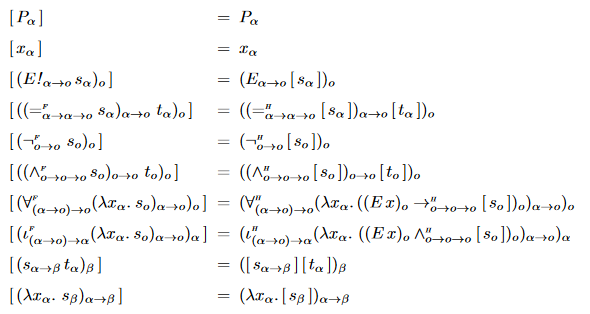
\includegraphics[scale=0.4]{images/embedding.png} 
\end{center}
\end{frame}

%------------------------------------------------------------------------------------
\section{Farmer's Approach}\label{farmer}

\begin{frame}
\begin{center}
\Large [ Approach \ref{farmer} ]\bigskip

Farmer's ``Traditional Approach''
\normalsize
\end{center}
\end{frame}

\begin{frame}
\frametitle{Farmer's ``Traditional Approach''}
The \IMPS /\LUTINS (and similarly, CASL) approach to undefinedness is as follows:
\bigskip

\textbf{Partial valuation for individuals, total valuation for formulas!}
\bigskip

That means \emph{formulas are always true or false}, and hence, always defined. Should a subterm of the equation be undefined, the formula denotes false.
\pause\bigskip

Some consequences:

\footnotesize
$$\textcolor{ForestGreen}{\forall x, y, z : \mathbb{R} \; . \; x = \frac{z}{y} \Rightarrow x \cdot y = z} \quad // \quad
\textcolor{red}{\forall a, b : \mathbb{R} \; . \; \neg \left(a \leq \frac{1}{b}\right) \equiv \left(a > \frac{1}{b}\right)}$$
\normalsize
\end{frame}

\begin{frame}
\frametitle{Undefinedness in \IMPS}

The chosen approach to undefinedness leads to pleasant results:
\medskip

\begin{itemize}
\item $x + \frac{1}{x}$ and $\left( \frac{1}{x}\right)^2$ do not have values if the value of $x$ is $0$.\medskip

\item If $\varphi\prime$ is the result of replacing $\left(\frac{1}{x}\right)^2$ with $\frac{1}{x^2}$ in $\varphi$, then $\varphi$ and $\varphi\prime$ are equivalent regardless of the value of $x$.\medskip

\item The equation $\sqrt{x} = 2$ over $\mathbb{R}$ is true for $x = 4$ and false everywhere else, even for $x < 0$.\medskip
\end{itemize}
\medskip

\dots which are typical of statements from chalk-and-blackboard mathematics.
\end{frame}

\begin{frame}
\frametitle{Example: Quasi-Equality}

This approach makes it easy to handle undefinedness, when it becomes necessary to deal with.\medskip

For example, regular equality (a formula like $E_1 = E_2$) can easily be extended into quasi-equality ($E_1$ and $E_2$ are quasi-equal iff they are either both defined and equal or they are both undefined) since reasoning about definedness is allowed and natural:

$$E_1 \simeq E_2 \;\equiv\; (\defined{E_1} \vee\, \defined{E_2}) \Rightarrow E_1 = E_2$$
\end{frame}

%------------------------------------------------------------------------------------
\section{Conclusion}

\begin{frame}
\frametitle{Conclusion}
Some takeaway messages from this are:
\bigskip

\begin{itemize}
\item Undefinedness in mathematics is interesting and ubiquitous.
\item Hence, we want it in our formal systems, but we don't, yet.
\item There's no \emph{one correct way} to do undefinedness!
\end{itemize}
\end{frame}

\begin{frame}
\frametitle{Sources}
\vfill
\begin{center}
\url{https://kwarc.info/public/proposal_jbetzendahl.pdf}
\medskip

\emph{Full bibliography available upon request.}
\end{center}
\vfill
\end{frame}

\end{document}